\documentclass{../qh_exercise}
\graphicspath{ {./images/} }

\begin{document}

\section{Leerdoelen}
\begin{itemize}
\item Omgaan met classes en objecten
\item Particles maken en updaten
\end{itemize}

\section{Uitleg}
\begin{itemize}
\item \myhref{https://natureofcode.com/book/chapter-4-particle-systems/}{Particle Systems - The Nature of Code}\\
    Alleen \textbf{4.1, 4.2, 4.3, 4.4, 4.5}
    \item \myhref{https://www.youtube.com/watch?v=vdgiqMkFygc&list=PLRqwX-V7Uu6Z9hI4mSgx2FlE5w8zvjmEy&index=1}{Chapter 2. Particle Systems}\\
    Alleen \textbf{4.1, 4.2, 4.3, 4.4, 4.5}\\
\end{itemize}

\section{Voorbeelden}
\begin{itemize}
    \item rain
\end{itemize}

\newpage
\section{Opdrachten}
In deze opdracht ga je \textbf{vuur} maken! Dit gaan je doen door een \textbf{particle system} te maken (zie uitleg en figuur \ref{fig:fire}).

\begin{figure}[H]
	\centering
	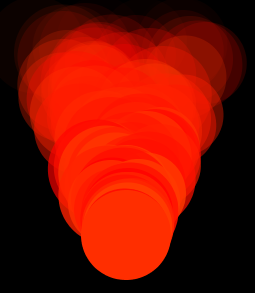
\includegraphics[width=6cm]{fire.png}
	\caption{Vuur!}
	\label{fig:fire}
\end{figure}

\subsection{Een particle}
Maak een \textbf{Particle} class. Bedenk zelf welke variabelen en methods deze class waarschijnlijk moet hebben. Kijk naar figuur \ref{fig:fire}, welke eigenschappen heeft \'e\'en vuur-deeltje?

\subsection{Het tekenen}
Maak een ArrayList van particles en zorg ervoor dat alle particles.
Voeg hier \'e\'en particle aan toe (in de \texttt{setup} functie).
Zorg er vervolgens voor dat alle particles getekent worden (doe dit dus uiteraard in de \texttt{draw} method).

\subsection{Het updaten}
Maak een \texttt{update} method in \texttt{particle} die ervoor zorgt dat de deeltjes omhoog vliegen en een klein beetje naar links of rechts
\remark{Het is hier dus super handig als je gebruik maakt van een \textt{PVector}}

\subsection{Lifetime}
We willen dat \'e\'en vuurdeeltje na een tijdje verdwijnt. Dit kun je doen door een variable \texttt{float lifetime = 255;} te maken. Elke update haal je hier \texttt{1} vanaf \texttt{lifetime--;}. Vervolgens moet je tijdens het updaten checken of \texttt{lifetime < 0}. Is dit het geval, dan moet je het deeltje uit de ArrayList halen (\texttt{particles.remove(particle)}, waar \texttt{particles} de ArrayList is, en \texttt{particle} het deeltje wat je wil weghalen).

\subsection{Kleur veranderen}
Zorg ervoor dat de vuur deeltjes meer doorzichtig worden naarmate ze korter te leven hebben.
\tip{Gebruik \texttt{fill(color,alpha)} waar bijvoorbeeld \textt{color = color(255,50,0)} en \textt{alpha} tussen \textt{0} en \texttt{255}}

\subsection{Vuur!}
Voeg elke keer dat \textt{draw} wordt aangeroepen een nieuwe particle toe aan de ArrayList zodat een prachtig vuur ontstaat!

\subsection{Extra mooi vuur}
Als je wil kun je ook nog extra dingen toevoegen:
\begin{itemize}
    \item Dat de grote van de vuur deeltjes verschillend is
    \item Dat de kleur van de vuur deeltjes verschillend is
    \item Dat het vuur je muis volgt
    \item Dat je meerdere vuurtjes kunt maken
\end{itemize}

\end{document}